% https://dvmarcilio.github.io/papers/icpc2019.pdf
% http://aagasc.edu.in/cs/books/Software%20Quality%20Assurance%20From%20Theory%20to%20Implementation.pdf
% see document in Downloads!

\section{Softwarequalität}\label{softwarequality}
In der DIN-ISO-Norm 9126 wird Software Qualität so definiert:
\dq Software-Qualität ist die Gesamtheit der Merkmale und Merkmalswerte eines Software-Produkts, die sich auf dessen Eignung beziehen, festgelegte Erfordernisse zu erfüllen.\dq

\citeauthor{hoffmann2013software} (\citeyear{hoffmann2013software}) hebt zu dieser Definition hevor, dass es nicht ein einziges Kriterium gibt, welches die Qualität von Software misst.
Vielmehr ist es eine Kombination verschiedener Kriterien.
Auf diese wird im folgenden Abschnitt (\ref{kriterien}) eingegangen.
Die Software-Qualitätssicherung befasst sich mit Methoden welche eingesetzt werden können, um bei diesen Kriterien gut abzuschneiden.
Sie wird im Abschnitt \ref{qualisicherung} behandelt.

\subsection{Kriterien}\label{kriterien}
In den folgenden Abschnitten werden die Kriterien erklärt, welche nach \citeauthor{hoffmann2013software} relevant sind für die Softwarequalität.
Die ersten vier Kriterien sind dabei für den Kunden wichtig, da diese direkte Auswirkung auf ihn haben.
Die letzteren vier sind nur für den Hersteller der Software relevant.
\subsubsection{Funktionalität}
Die Funktionalität gibt an, ob die spezifizierten Anforderungen erfüllt sind.
Funktionale Fehler werden meist durch Bugs in der Implementierung verursacht, können ihren Ursprung jedoch auch in fehlenden oder falsche verstandenen Spezifikationen haben.
Sie können durch den Einsatz von Software-Qualitätsicherungstools vorgebeugt werden.

\subsubsection{Performance}
Mit Performance sind die Anforderungen an die Software während deren Laufzeit gemeint.
Für einfache Desktop Anwendungen stellt dieses Kriterium meist kein Problem dar.
Handelt es sich bei der Anwendungen jedoch um ein Echtzeitsystem, so ist die Performance eines der wichtigsten Kriterien.

\subsubsection{Zuverlässigkeit}
Mit diesem Kriterium ist gemeint, wie zuverlässig eine Software ihre Funktionen ausführt.
Kommt es oft zu Fehlern oder Abstürzen, so ist die Zuverlässigkeit tief.
Sie ist stark an die anderen Kriterien gekoppelt.
Hat die Software inkorrekte Funktionalität oder schlechte Performance, so ist auch die Zuverlässigkeit tief.

\subsubsection{Benutzbarkeit}
Die Eigenschaften einer Software, welche mit dem Menschen interagieren, sind in diesem Kriterium zusammengefasst.
Im Abschnitt \ref{usability} wird diese Thematik vertieft.

\subsubsection{Wartbarkeit}
Um eine Software auch nach der ersten Inbetriebnahme weiter zu entwickeln, muss diese Wartbar sein.
Es soll möglich sein, erkannte Bugs einfach zu beheben.
Die Software soll so aufgebaut sein, dass sie nicht vollständig umgebaut werden muss, nur um eine neue Funktion hinzuzufügen.


\subsubsection{Transparenz}
Mit diesem Kriterium wird bewertet, wie transparent das Program intern umgesetzt ist.
Alle Teilkomponenten der Software sollen einfach zu verstehen sein.
Tendenziell verschlechtert sich die Transparenz im Verlaufe der Weiterentwicklungen.


\subsubsection{Übertragbarkeit}
Die Übertragbarkeit gibt an, ob sich eine bestehende Software in eine andere Umgebung übertragen lässt.
Kann ein Programm nur auf einer bestimmten Betriebssystemversion oder gar nur auf einem einzigen Rechner ausgeführt werden, so ist dessen Übertragbarkeit sehr schlecht.
Mit Umgebung ist jedoch nicht nur die technische Umgebung wie das Betriebssystem gemeint, sonder sie kann auch Aspekte wie die Sprache oder Kultur beinhalten.

\subsubsection{Testbarkeit}\label{testability}
Software ist meist so komplex, dass es nicht ausreicht, lediglich die Benutzerschnittstellen zu testen.
Die möglichen Kombinationen von Eingabeparametern sind dabei viel zu umfangreich.
So müssen einzelne Komponenten einzeln getestet werden.
Dies ist nur möglich, wenn diese so entwickelt werden, dass sie auch testbar sind.
Damit ist gemeint, dass bspw. ein Algorithmus so implementiert ist, dass er von keinerlei internen Zuständen der Anwendungen abhängig ist. 


\subsection{Software-Qualitätssicherung}\label{qualisicherung}
Unter Software-Qualitätssicherung versteht sich eine systematische und geplante Sammlung von Aktionen, 
welche die Sicherheit geben, dass die erstellte Software den Anforderungen entspricht.
Diese sollen den Entwicklungsprozess evaluieren und sicherstellen,
dass die Software im gegebenen zeitlichen sowie finanziellen Rahmen erstellt werden kann \parencite{galin2004software}. 

Sie unterscheidet sich von der Qualitätskontrolle indem sie nicht das fertige Produkt sondern den Herstellungsprozess evaluiert und prüft \parencite{galin2004software}.
Die beiden Teile, Produktqualität und Prozessqualität, aus welchen sich die Software-Qualitätssicherung nach \citeauthor{hoffmann2013software} zusammensetzt, werden in den nächsten Abschnitten erläutert.

\subsection{Produktqualität}
Zur Sicherung der Produktqualität gehören jene Ansätze welche einen direkten Einfluss auf das Produkt und somit auf die zuvor genannten Kriterien haben.
In nächsten Abschnitten werden einige Techniken und Methoden erklärt, welche laut \citeauthor{hoffmann2013software} bei der Sicherung der Produktqualität helfen.

\subsubsection{Software-Richtlinien}\label{quality_richtline}
Software-Richtlinien sind Konventionen, welche vorgeben, wie mit einer bestimmten Programmiersprache gearbeitet werden soll.
Sie befassen sich dabei mit jenem Teil, welcher von der Syntaktik und Semantik einer Sprache nicht vorgegeben ist.
Ihr Ziel ist es, die geschriebene Software zu vereinheitlichen.
Dies verhindert, dass die Teile einer Software in unterschiedlichen Programmierstilen geschrieben sind, in welche sich jeweils mit viel Zeitaufwand eingearbeitet werden muss.
Des Weiteren sollen sie zu Fehlerreduktion führen, indem einheitliche Lösungsmuster vorgeschrieben werden sowie fehleranfällige Sprachkonstrukte verboten werden.

Die folgenden Punkte sind Beispiele, welche in einer typischen Richtlinie vorhanden sein können:
\begin{itemize}
   \item Die Schreibweise von Bezeichnern (z.B. Pascal Case)
   \item Die Verwendung von Einrückungen, Leerzeichen und Zeilenschaltungen
   \item Vorgaben, welche Codeteile wie dokumentiert werden
\end{itemize}
Einige Konventionen, wie beispielsweise die \textit{MISCRA-C}\footnote{https://www.misra.org.uk/} Sprachkonvention, geben des Weiteren konkrete Vorgaben zur Verwendung bestimmter Sprachkonstrukte an.
In Abbildung \ref{fig:misra} ist ein Ausschnitt aus \textit{MISCRA-C} abgebildet.
\begin{figure}[H]
   \centering
   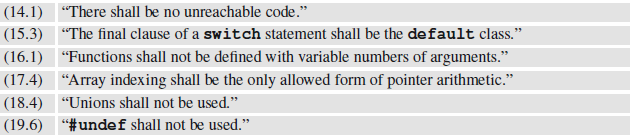
\includegraphics[width=1.0\textwidth]{gfx/misra.png}
   \caption{
      Ausschnitt aus der \textit{MISCRA-C} Sprachkonvention
   }
   \source{\cite{hoffmann2013software}}
   \label{fig:misra}
\end{figure}


\subsubsection{Typisierung}\label{typing}
Die Verwendung eines Typisierungssystem steigert die Qualität einer Software.
Mittels statischer Typprüfung wird durch den Compiler geprüft, ob die verwendeten Typen jeweils korrekt sind.
Die dynamische Typprüfung, welche meist von einem Interpreter durchgeführt wird, erkennt falsch verwendete Typen bei Laufzeit und kann so Programmabstürze verhindern.

Viele Programmiersprachen bieten eine statische oder dynamische Typprüfung an.
Einige, wie bspw. C\#, sogar beide.

\subsubsection{Portabilität}\label{portability}
Bei der Portabilität geht es nicht direkt darum, dass eine Software auf allen erdenklichen Systemen läuft, sondern vielmehr, dass die Portierung auf ein neues System mit geringem Aufwand vollbracht werden kann.
Dazu gehört, dass nur jene Codeteile angepasst oder neu geschrieben werden müssen, welche effektiv eine Abhängigkeit zum jeweiligen System haben.
Die Businesslogik einer Anwendung ist typischerweise eher unabhängig von einem System, während die Benutzerschnittstelle stark an ein bestimmtes Betriebssystem gekoppelt sein kann.
Um die Portabilität zu gewährleisten, soll der Code von Anfang an so organisiert werden, dass plattformunabhängige Komponenten sauber von den plattformabhängigen getrennt sind.

\subsubsection{Fehlertolerante Programmierung}
Software-Systeme reagieren unterschiedlich auf Fehler.
Bei Desktop Anwendungen im Büroumfeld ist der Absturz einer Anwendung nicht vorteilhaft, wird jedoch von Nutzern akzeptiert.
Bei sicherheitskritischen Systemen ist dies nicht der Fall.
Software, welche bswp. die Unversehrtheit von Personen tangieren, muss so programmiert werden, dass sie mit Fehlern umgehen kann.
Ein Ansatz dazu ist, dass Teile des Systems mehrfach vorhanden sind.
Diese Redundanz führt dazu, dass ein Ausfall eines Teiles nicht zum Absturz des ganzen Systems führt.

Bei jeder Art von Software ist die Ausnahmebehandlung da, um mit spontan aufgetretenen Fehlern umzugehen.
Geplante Ausnahmen, wie beispielsweise ungültige Eingaben eines Nutzers, können behandelt und dem Benutzer entsprechend mitgeteilt werden.
Ungeplante Ausnahmen, wie beispielsweise eine Division durch Null, können behandelt werden, um einen Absturz des Programms zu verhindern.


\subsubsection{Software-Test}\label{quality_test}
Bei Software-Tests wird eine Komponente mit vordefinierten Eingabewerten und bestimmten Zuständen ausgeführt.
Das Ergebnis wird mit einem Erwartungswert abgeglichen.
So kann sichergestellt werden, dass eine Komponente so funktioniert, wie sie soll.
Da Tests nicht nur auf der Ebene einer einzelnen Komponente geschrieben und ausgeführt werden können, sondern auch das Zusammenspiel mehrerer Komponenten oder ganzer Systeme testen können,
sind sie für das Kriterium der Funktionalität sehr wichtig.
Sie sind somit ein wichtiger Bestandteil eines Softwareprojekts.
%todo evtl schreiben, dass tests selbst hohe quali haben müssen
Während des Schreibens von Tests zeigt sich auch, zu welchem Grad das Kriterium der Testbarkeit erfüllt ist.

Testmetriken geben Auskunft zu einer Testmenge.
Sie geben an, ob eine Komponente ausreichend getestet wurde und welche Teile des Codes noch nicht getestet sind.

\subsubsection{Statische Analyse}
Im Gegensatz zu den im vorherigen Abschnitt erwähnten Software-Tests wird bei der statischen Analyse der zu bewertende Code nicht ausgeführt.
Vielmehr werden Aspekte des Codes systematisch quantitativ erfasst.
Dies wird automatisiert mit einer entsprechenden Software gemacht und kann folgende Punkte beinhalten:
\begin{itemize}
   \item Metriken, welche die Software in Punkten wie beispielsweise Komplexität, Wartbarkeit oder Kohäsion beurteilen.
   \item Überprüfung, ob Software-Richtlinien eingehalten wurden.
   \item Erkennen von Anomalien oder Sicherheitslücken im Code.
\end{itemize}

Im Abschnitt \ref{quality:sonar} wird das Programm SonarQube vorgestellt, welches für solche statischen Analysen eingesetzt werden kann.

\subsection{Prozessqualität}
Die in den folgenden Abschnitten erklärten Massnahmen zur Verbesserung der Prozessqualität haben keinen direkten Einfluss auf die Qualitätskriterien.
Vielmehr bilden sie eine Grundlage um überhaupt qualitative Software erstellen zu können.

\subsubsection{Build- \& Test-Automatisierung}
Bei der Build- \& Test-Automatisierung geht des darum, dass das Kompilieren der Software sowie das Ausführen von Software-Tests ohne manuellen Aufwand auf einem Server ausgeführt wird.
Dies kann beispielsweise bei jedem Commit oder jeder neuen Version der Software geschehen.
Das Ziel dabei ist, dass neue Defekte möglichst rasch erkannt werden.
Werden die Testresultate über einen längeren Zeitraum abgelegt, so lassen diese Rückschlüsse auf die Stabilität einzelner Softwarekomponenten zu.

\subsubsection{Vorgehensmodelle}
Als Vorgehensmodell soll eine bewährte Methodik gewählt werden, welche vorgibt, wie das Softwareprojekt konkret umgesetzt wird.


\subsubsection{Versionsverwaltung}
Ein Versionsverwaltungsystem ist ein Repository, welches alle Artefakte, die zur Erstellung der Software benötigt werden, speichert und bei Änderungen deren Versionen verwaltet.
Bei einem solchen System sind unter anderem folgenden Punkte wichtig:
\begin{itemize}
   \item Die gemachten Änderungen sollen transparent protokolliert sein.
   \item Es soll möglich sein, jederzeit auf ältere Versionen des Codes zuzugreifen.
   \item Entwickler müssen gleichzeitig am selben Code arbeiten können.
\end{itemize}



\subsection{SonarQube}\label{quality:sonar}
SonarQube ist ein Software-Qualitatssicherungstool, welches Code analysiert und Berichte zur Codequalität erstellt.
Die Berichte könne beispielsweise Code-Style-Verletzungen, Designfehler oder gar Sicherheitslücken aufzeigen.
Da die Analysen statisch sowie dynamisch durchgeführt werden, können auch Metriken zu Codeabdeckung durch Tests erstellt werden \parencite{malloy_2021}.
SonarQube berichtet nicht nur über erkannte Probleme, sondern beinhaltete auch Funktionen um diese zu verwalten.
Ein Problem kann beispielsweise direkt der Person zugewiesen werden, welche es bearbeiten soll.
Meldungen, welche nicht bearbeitet werden, können entsprechend markiert werden, so dass sie in Zukunft nicht erneut auftreten.
Da SonarQube die Historie der Berichte speichert, werden neue Probleme speziell hervorgehoben.
Wie sich die totale Anzahl der Probleme über die Zeit entwickelt, wird ebenfalls angezeigt und gibt einen Trend der Softwarequalität an.

% Maintainability, Security, Reliability, Complexity

\subsubsection{Funktionsweise}\label{sonar:funktionsweise}
In einem produktiven Umfeld ist die Funktionsweise von SonarQube wie folgt:
SonarQube wird auf einem Server installiert und mit einem \ac{CI} Server verbunden.
Wenn Entwickler Änderungen am Code in das jeweilige \ac{SCM} System pushen, löst dies einen Build auf dem \ac{CI} Server aus.
Dieser Build beinhaltet Sonar Scanner.
Ist der Build abgeschlossen, werden die Berichte der Scanner an die SonarQube Instanz übermittelt.
Dort werden sie verarbeitet, in der Datenbank abgelegt und über eine Benutzerschnittstelle dargestellt \parencite{malloy_2021}.

\subsection{Qualitätssicherungstools bei der Landis+Gyr}
Für die Qualitätssicherung der Firmware setzt die Landis+Gyr aktuell C-STAT\footnote{https://www.iar.com/cstat} für statische Codeanalysen ein.
Eine kürzlich durchgeführte Evaluation hat jedoch ergeben, dass SonarQube die geeignetere Lösung wäre.
Dieser Umstieg ist zum Zeitpunkt dieser Arbeit bereits geplant, jedoch noch nicht realisiert.
Bei den verschiedenen C\# Projekten, welche in diesem Kapitel genannt wurden, werden keinerlei Qualitätsicherungstools eingesetzt.
